\section{GUI-Library}
Agrupadas bajo un mismo \emph{namespace} estas clases representan cada uno de los componentes que pueden formar parte del interfaz de usuario.\\
\begin{figure}[h]
	\centering
		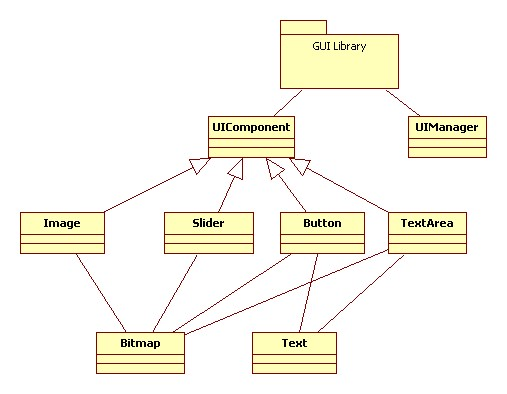
\includegraphics[width=10cm]{images/diagramas/gui.jpg}
	\caption{Diagrama de GUI Library}
	\label{fig:gui-library}
\end{figure}

Las caracter�sticas principales de la biblioteca gr�fica son:
\begin{itemize}
	\item Todos los componentes heredan de UIComponent.
	\item Se ha buscado el menor acoplamiento posible con la tecnolog�a usada para el rendernizado y computar de eventos de rat�n (DirectX).
	\item Todos los componentes utilizan la funcionalidad m�nima de dos entidades m�s primitivas: Bitmap y Text. Se puede decir que todos los componentes son \emph{composiciones} de un n�mero variable de estos elementos, dot�ndolos luego del comportamiento acorde a su naturaleza.
	\item La gesti�n de todos los componentes pasa por una sola clase (UIManager).
	\item El sistema es muy rudimentario pero funcional: se cargan todos los componentes desde el inicio de la ejecuci�n, manteni�ndolos ocultos o visibles seg�n necesidad.
	\item El esta del interfaz de usuario es global, es decir, compartido por todos los componentes del mismo.
\end{itemize}

\subsection{UIComponent}
UIComponent representa el comportamiento y funcionalidad b�sica de todo componente del interfaz de usuario. Todo elemento del interfaz \emph{es un UIComponent}. Esto puede llevar a pensar que UIComponent deber�a ser una clase abstracta, pero la implementaci�n es m�s clara y ofrece mayores posibilidades si esto no se hace.\\

Las caracter�sticas principales de todo UIComponent son:

\begin{figure}[h]
	\centering
		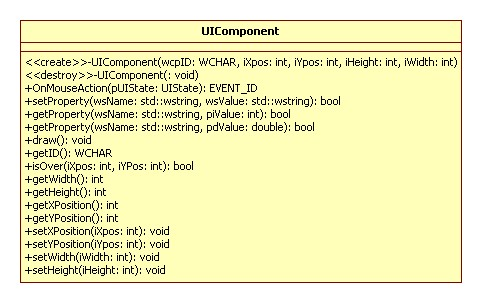
\includegraphics[width=15cm]{images/diagramas/uicomponent.jpg}
	\caption{Diagrama de clase de UIComponent}
	\label{fig:uicomponent}
\end{figure}

\begin{itemize}
	\item Ocupa una \emph{posici�n} en la pantalla. 
	\item Tiene un \emph{tama�o}.
	\item Recibe \emph{eventos} previamente procesados por el UIManager y devuelve otros de acuerdo a su naturaleza.
	\item Tiene dos estados: uno corresponde al momento de ser interactuado (\emph{Hot}) y otro cuando se produce dicha interacci�n (\emph{Active}).
	\item Tiene un \emph{identificador} �nico dentro el interfaz gr�fico de usuario.
	\item Se puede acceder al estado intr�nseco del objeto (sus atributos) de una forma est�ndar: mediante la llamada a un m�todo que recibe como par�metro el identificador de dicho atributo.
	\item Se puede variar el estado intr�nseco del objeto (sus atributos) de una forma est�ndar: mediante la llamada a un m�todo que recibe como par�metro el identificador de dicho atributo.
	\item Tiene la capacidad de dibujarse.
\end{itemize}


\subsection{UIManager}

\begin{figure}[h]
	\centering
		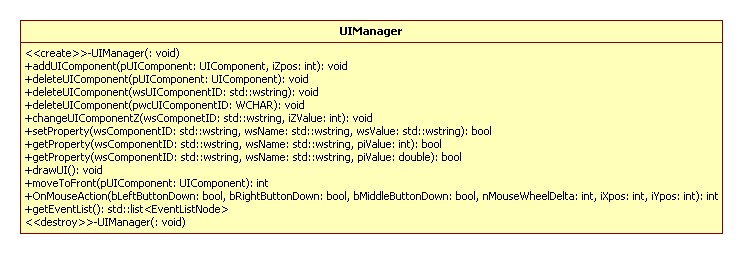
\includegraphics[width=15cm]{images/diagramas/uimanager.jpg}
	\caption{Diagrama de clase de UIManager}
	\label{fig:uicomponent}
\end{figure}